\author{Gottfried von Recum}
\section{Zeitplanung}

Um alle Aufgaben bestmöglich erledigen zu können wird zunächst eine Zeitplanung erstellt. Diese gilt als Richtschnur und wird wiederkehrend überprüft.

\begin{figure}[ht]
    \centering
    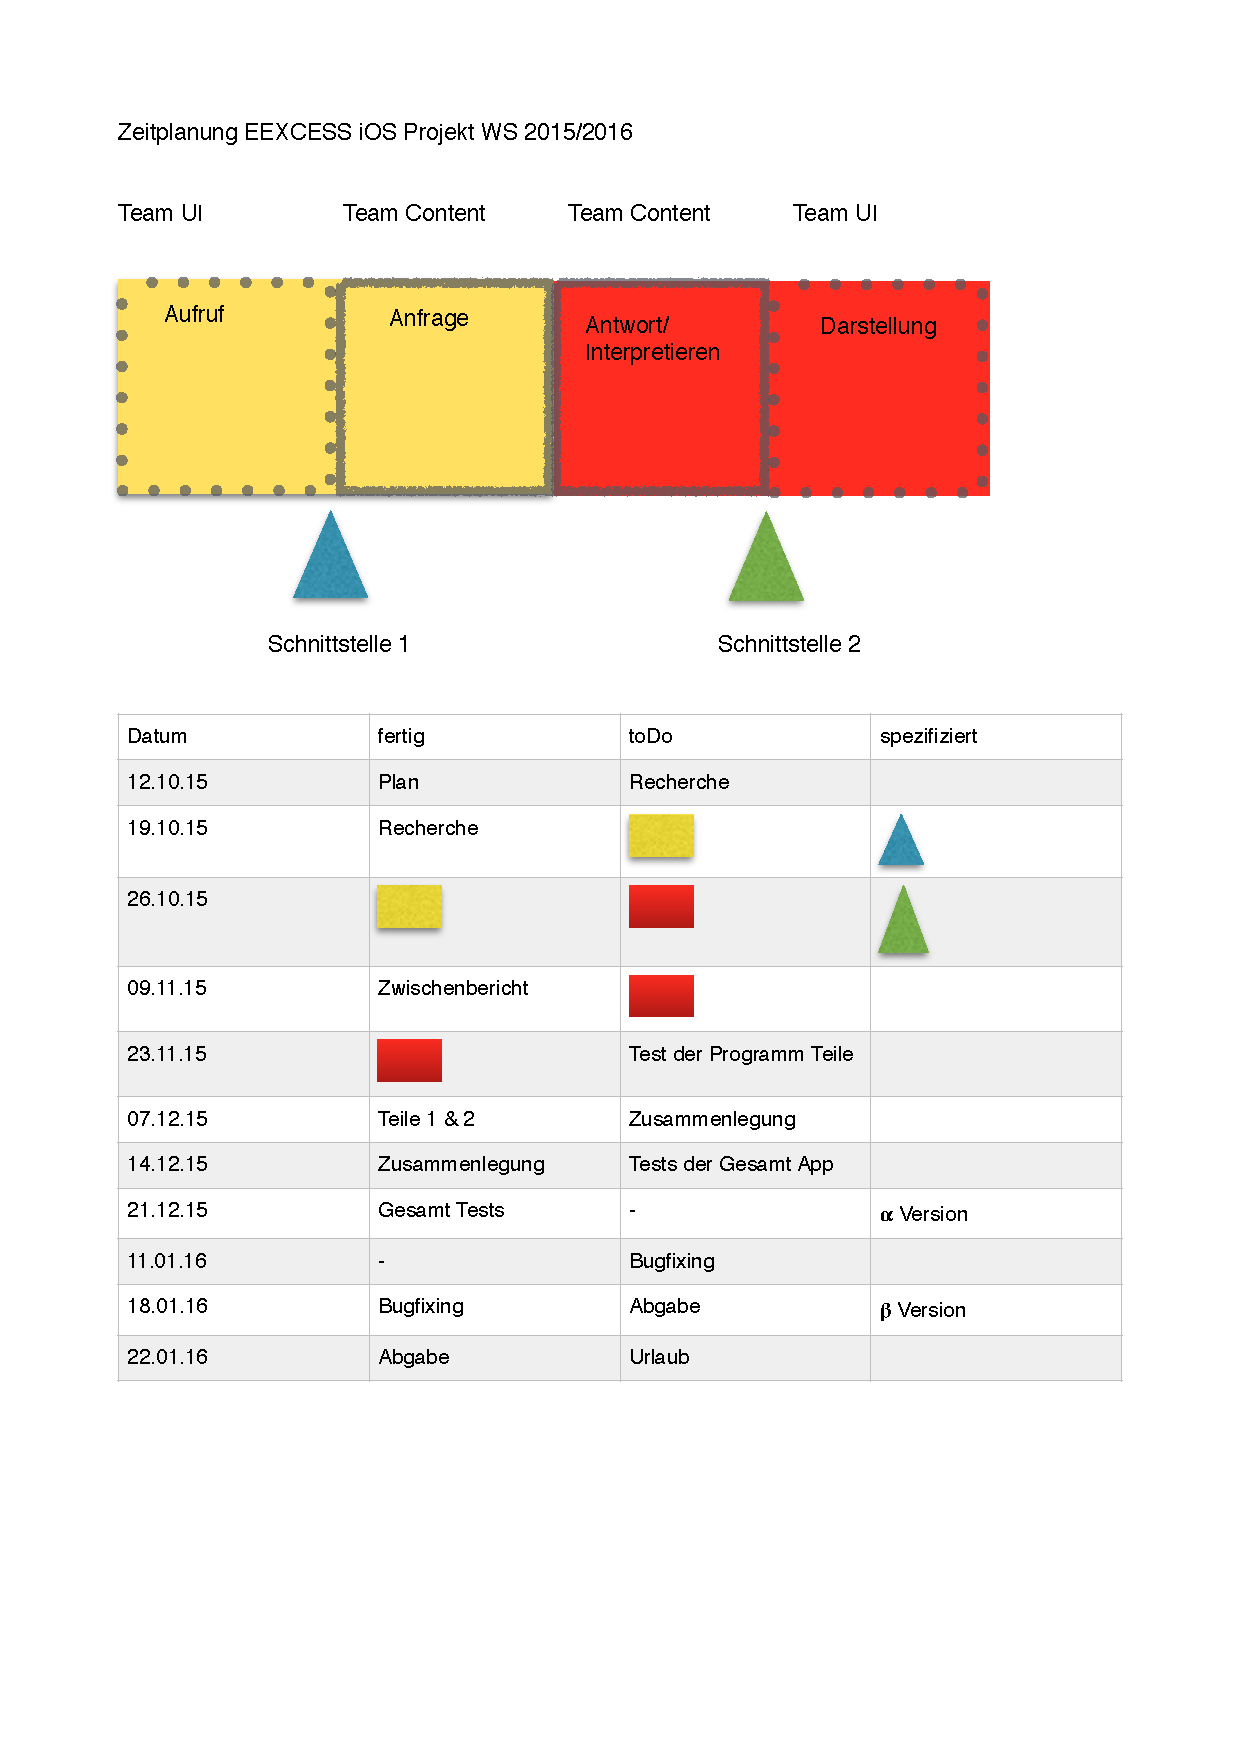
\includegraphics[width=0.735\textwidth]{Zeitplanung}
    \caption{Zeitplanung für das \SECH-Browser Projekt}
    \label{fig:Zeitplanung}
\end{figure}